%%% Local Variables:
%%% mode: latex
%%% TeX-master: t
%%% End:


\documentclass{article}
\usepackage[T1]{fontenc}
\usepackage[utf8]{inputenc}
\usepackage{amsmath}
\usepackage{amssymb}
\usepackage{hyperref}
\usepackage{parskip}
\usepackage{float}
\usepackage{graphicx}
\usepackage{listings}
\usepackage{cleveref}
\usepackage{circuitikz}
\usepackage{listings}

\title{Design of Digital systems 1 TFE4141 - Assignment 4}
\author{Sindre Hansen - 732719}
\date{Fall 2016}

\renewcommand\thesection{\arabic{section}}
\renewcommand\thesubsection{\thesection.\arabic{subsection}}


\begin{document}
\begin{figure}
  \centering
  
\includegraphics[width=0.5\textwidth]{images/logontnu_eng}
\end{figure}
\maketitle
\rule{\linewidth}{0.5mm}

\section{Task 1}
\subsection{}
\begin{figure}[hbp]
  \centering
  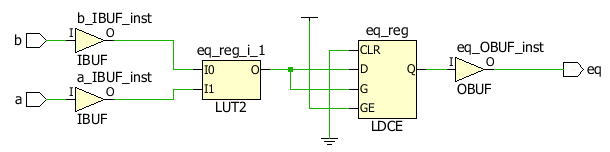
\includegraphics[width=\textwidth]{images/task1-1}
\end{figure}

\subsection{}
An example where a latch is unintentionally created is when you don't
assign values to all output in every branch of an if-statement.

\subsection{}
The way to make sure that latches are not generated from combinatorial
processes is to always make sure that there are no incomplete
branches, or incomplete signal assignments.

\section{Task 2}
\subsection{}
If we assume that on the first run the reset is held high then there's
created a single flip-flop for 't' in both designs. However, if we on
the next run assume that the reset is low, the difference in the two
designs become clearer. Since design1 has the signal assignment before
the variable assignment it needs to create another flip-flop for
't'. Therefore we end up with two flip-flops in the synthesis.

Design2 has the signal assignment after the variable assignment and
therefore we end up with just one flip-flop in the synthesis.

\subsection{}
Image: task2-design1

Image: task2-design2

\subsection{}
There are two main requirements for a variable to be implemented as a
register. One, it needs to be dependent of a clock and two, a variable
needs to be assigned to a signal.

If you alter the variable after the last assignment to the signal a
new register is created. It is this that happens in design1.

\subsection{}
A variable is local to each process, its scope does not extend beyond
the process. As such one can not read or write to it from another
process. A signal is defined outside of the process and therefore
it can safely be read from multiple processes. If one wishes to write
to the signal you need to be careful with avoiding conflicts.

\section{Task 3}
\subsection{}
The reason that the process is not synthesizable is due to a security
feature in Vivado. The reason for this security feature is to minimize
differences between simulation and synthesis.

\subsection{}
Yes, there is reason to suspect a difference between simulation and
synthesization. The reason is that the synthesized circuit will be
sensitive to signals that the simulation is not.

\subsection{}
Make sure that every sensitivity list is updated with all signals it
needs to react to.









\end{document}
